\newpage
\section{Deep Boltzmann Machines \cite{salakhutdinov2013learning, salakhutdinov2009deep, goodfellow2016deep}}
\subsection{More efficient learning algorithm for general binary-binary BMs}
\subsubsection{PCD-k}
To recap:
\bg
\frac{1}{N}\sum_{n=1}^N\nabla_{\mb{W}}\log p(\mb{x}_n;\bs{\psi}) = \E_{\mb{v},\mb{h}\sim P_{\text{data}}(\mb{v},\mb{h};\bs{\psi})}\l[\mb{v}\mb{h}^T\r]-\E_{\mb{v},\mb{h}\sim P_{\text{model}}(\mb{v},\mb{h};\bs{\psi})}\l[\mb{v}\mb{h}^T\r]
\eg
and similar formulae for log-likelihood gradients w.r.t. $\mb{L},\mb{J},\mb{b},\mb{c}$, see (17).
\\[0.5em]
Now, instead of CD-k we use PCD-k (i.e. we keep one Markov chain without restarting its state between the updates), which falls into class of so-called \emph{Stochastic approximation procedures} (SAP) to estimate \tb{model's} expectations.
\\[1em]
Let $\bs{\psi}^t$ and $\mb{x}^t$ be the current model parameters and the state. Then $\mb{x}^t$ and $\bs{\psi}^t$ are updated sequentially as follows:
\begin{itemize}
	\item given $\mb{x}^t$, a new state $\mb{x}^{t+1}$ is sampled from a transition operator $T_{\bs{\psi}^t}(\mb{x}^{t+1}\leftarrow \mb{x}^t)$ that leaves $p(\cdot,\cdot;\bs{\psi}^t)$ invariant (which in our case is performing Gibbs sampling using equations (11) and (12) for $k$ steps);
	\item a new parameter $\bs{\psi}^{t+1}$ is then obtained by replacing the intractable model's expectation by the point estimate $\mb{x}^t$ (see also subsubsection 2.2.2 for whether to sample or use probabilities/means instead of sampling, and for which type of states)
\end{itemize}
In practice, we typically maintain a set of $P$ "persistent" sample "particles" $X^t=\{\mb{x}_1^t\ldots \mb{x}_{P}^t\}$ and use average over those particles.
\\[1em]
The intuition behind why this procedure works is the following: as the learning rate becomes sufficiently small compared with the mixing rate of the Markov chain, this "persistent" chain will always stay very close to the stationary distribution even if it is only run for a few MCMC updates per parameter update.
\\[1em]
Provided $\|\bs{\psi}^t\|$ is bounded and Markov chain, governed by a transition kernel $T_{\bs{\psi}^t}$ is ergodic (which is typically true in practice), and sequence of learning rates $\alpha_t$ satisfies $\sum_{t}\alpha_t=\infty$, $\sum_{t}\alpha_t^2<\infty$, this stochastic approximation procedure procedure is almost surely convergent to an asymptotically stable point.
\\
Note that in practice, $\alpha_t$ is not approached to zero, but rather to some small but positive constant $\varepsilon$ (e.g. $10^{-6}, 10^{-5}$).
\subsubsection{Variational learning}
Another approach is used to approximate \tb{data}-dependent expectations. We approximate true posterior over latent variables $p(\mb{h}|\mb{v};\bs{\psi})$ (which is intractable in general BM, tractable in RBM, but will be again intractable in DBM) by approximate posterior $q(\mb{h};\bs{\mu})$ and the variational parameters $\bs{\mu}$ are updated to follow the gradient of a \emph{lower bound on the log-likelihood}:
\\[1em]
In general:
\begin{empheq}[box={\mybox[1em][1em]}]{gather*}
\log p(\mb{v};\bs{\psi})=\int q(\mb{h};\bs{\mu})\log p(\mb{v};\bs{\psi})\mathrm{d}\mb{h}
=\int q(\mb{h};\bs{\mu})\log \frac{p(\mb{v},\mb{h};\bs{\psi})}{p(\mb{h}|\mb{v};\bs{\psi})}\mathrm{d}\mb{h}=\\
=\int q(\mb{h};\bs{\mu})\log \l(\frac{p(\mb{v},\mb{h};\bs{\psi})}{q(\mb{h};\bs{\mu})}\cdot \frac{q(\mb{h};\bs{\mu})}{p(\mb{h}|\mb{v};\bs{\psi})}\r)\mathrm{d}\mb{h}=\\
=\int q(\mb{h};\bs{\mu})\log p(\mb{v},\mb{h};\bs{\psi})\mathrm{d}\mb{h}
\underbrace{-\int q(\mb{h};\bs{\mu})\log q(\mb{h};\bs{\mu})\mathrm{d}\mb{h}}_{\mc{H}(q)}
+\underbrace{\int q(\mb{h};\bs{\mu})\log \frac{q(\mb{h};\bs{\mu})}{p(\mb{h}|\mb{v};\bs{\psi})}\mathrm{d}\mb{h}}_{D_{\text{KL}}(q(\mb{h};\bs{\mu}) \;\|\; p(\mb{h}|\mb{v};\bs{\psi}))\geq 0}\geq\\
\geq \int q(\mb{h};\bs{\mu})\log p(\mb{v},\mb{h};\bs{\psi})\mathrm{d}\mb{h} + \mc{H}(q) =: \mc{L}_{\text{ELBO}}(\bs{\mu}; \bs{\psi})
\end{empheq}
For Boltzmann Machine:
\begin{empheq}[box={\mybox[1em][1em]}]{gather*}
\text{\textbullet{} }[1]=\sum_{\mb{h}} q(\mb{h};\bs{\mu})\l[-E(\mb{v},\mb{h};\bs{\psi})=-\log Z(\bs{\psi}) \r]-\underbrace{\log Z(\bs{\psi})}_{=\text{ const w.r.t.}\bs{\mu}}\cdot\underbrace{\sum_{\mb{h}} q(\mb{h};\bs{\mu})}_{=1}+\\
+\sum_{\mb{h}} q(\mb{h};\bs{\mu})\l[\sum_{j<k}L_{jk}v_jv_k +\sum_{l<m}J_{lm}h_lh_m +\sum_{j,l}W_{jl}v_jh_l+\sum_jb_jv_j+\sum_lc_lh_l  \r]=\\
=\sum_{l<m}J_{lm}\E_{\mb{h}\sim q(\mb{h};\bs{\mu})}[h_lh_m]+\sum_{j,l}W_{jl}v_j\E_{\mb{h}\sim q(\mb{h};\bs{\mu})}[h_l]+\sum_lc_l\E_{\mb{h}\sim q(\mb{h};\bs{\mu})}[h_l]+\text{const}
\end{empheq}
For Boltzmann Machine and fully-factorizable $q(\mb{h};\bs{\mu})=\prod_l q(h_l;\mu_l), q(h_l=1;\mu_l)=\mu_l$ (\emph{mean-field} approach):
\begin{empheq}[box={\mybox[1em][1em]}]{gather*}
\text{\textbullet{} }[1]=\sum_{l<m}J_{lm}\mu_l\mu_m+\sum_{j,l}W_{jl}v_j\mu_l+\sum_lc_l\mu_l+\text{const}
\\
\text{\textbullet{} }[2]=\mc{H}(q)=-\sum_{\mb{h}}q(\mb{h};\bs{\mu})\log q(\mb{h};\bs{\mu})=-\sum_{\mb{h}}q(\mb{h};\bs{\mu})\sum_{j}\log q(h_j;\mu_j)=\\
=-\sum_j \sum_{h_j\in\{0,1\}}q(h_j;\mu_j)\log q(h_j;\mu_j) \underbrace{\sum_{\mb{h}_{-j}}q(\mb{h}_{-j};\bs{\mu}_{-j})}_{=1}=-\sum_j \mu_j\log \mu_j+(1-\mu_j)\log(1-\mu_j)
\end{empheq}
\bg
\boxed{\mc{L}_{\text{ELBO}}(\bs{\mu}; \bs{\psi})=\sum_{l<m}J_{lm}\mu_l\mu_m+\sum_{j,l}W_{jl}v_j\mu_l+\sum_lc_l\mu_l-\sum_j \mu_j\log \mu_j+(1-\mu_j)\log(1-\mu_j)+\text{C}}
\eg
Let us maximize (55) for $\bs{\mu}$ for fixed $\bs{\psi}$:
\begin{empheq}[box={\mybox[1em][1em]}]{gather*}
0 \doteq \frac{\partial}{\partial\mu_{i}}\mc{L}=\underbrace{\comment{$l=i$}\sum_{m>i}J_{im}\mu_m+\comment{$m=i$}\sum_{l<i}J_{li}\mu_l}_{=\comment{$J_{ij}=J_{ji},J_{ii}=0$}\sum_l J_{il}\mu_l}+\sum_{j}W_{ji}v_j+c_i
-\log \mu_i-1+\log(1-\mu_i)+1
\\
\Leftrightarrow
\\
\text{sigm}^{-1}(\mu_i)=\log\frac{\mu_i}{1-\mu_i}=\sum_{l<i}J_{li}\mu_l+\sum_{j}W_{ji}v_j+c_i
\end{empheq}
\bg
\boxed{\mu_i\leftarrow \text{sigm}\l(\sum_{l<i}J_{li}\mu_l+\sum_jW_{ji}v_j+c_i\r)}
\eg
Note that this is exactly the formula for (12) for computing $p(h_j=1|\mb{v},\mb{h}_{-i})$ in BM! So, updates of variational parameters can be computed using Gibbs sampler. This is not a coincidence, but the same holds if replace types of units, use RBM or even DBM (see below)!
\\[1em]
Note, that this variational approach cannot be used to approximate model-expectations because of minus sign in formulae (54),(17). This would cause variational learning to change the parameters so as to \emph{maximize} $D_{\text{KL}}(q(\mb{h};\bs{\mu}) \;\|\; p(\mb{h}|\mb{v};\bs{\psi}))$.
\\[0.5em]
The naive mean-field approach was chosen because:
\begin{itemize}
	\gooditem its convergence is usually fast;
	\gooditem it is unimodal.
\end{itemize}
Note that in general, we don't have to provide a parametric form of the approximating distribution beyond enforcing the independence assumptions. The variational approximation procedure is generally able to recover the functional form of the approximate distribution \cite{goodfellow2016deep}.

\subsection{Deep Boltzmann Machine}
Again assume unless specifically mentioned that DBM contains all binary units.
\subsubsection{High-level overview}
\textbullet{} DBM is a deep generative model, that consists of a layer of visible units and a series of layers of hidden units.
\begin{figure}[h]
\begin{mdframed}
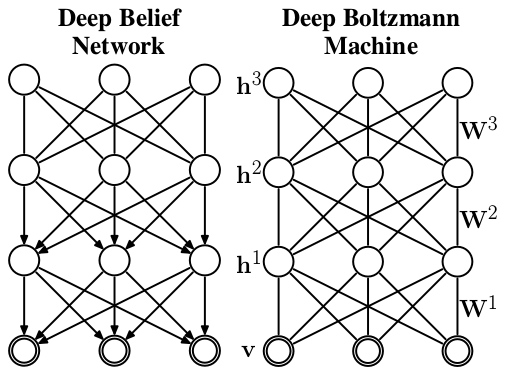
\includegraphics[scale=0.4]{img/dbn_dbm.png}
\centering
\caption{A three-layer Deep Belief Network and a three-layer Deep Boltzmann Machine.}
\label{fig:dbn_dbm}
\end{mdframed}
\end{figure}
In comparison to another deep generative model, DBN (which is hybrid, and has directed layers and one undirected), DBM is entirely undirected model, see Fig. \ref{fig:dbn_dbm}. DBN is trained using greedy, layer by layer training of corresponding RBMs (one bottom-top pass). At the same time, All parameters in DBM are learned \tb{jointly}, which greatly facilitates learning better generative models. Even though both models have a potential of learning series of internal representations that become increasingly complex, DBM's approximate bottom-top and top-bottom inference better propagate uncertainty $\Rightarrow$ deal more robustly with ambiguous inputs, than DBN.
\\
\textbullet{} Formally, suppose number of (hidden) layers $L=3$.
$$
\mb{v}\in\R^D, \mb{h}=\{\mb{h^{(1)}}, \mb{h^{(2)}}, \mb{h^{(3)}}\}, \mb{h^{(s)}}\in\R^{H_s}, s\in\{1,2,3\};
$$
Energy function:
\bg
E(\mb{v},\mb{h};\bs{\psi})=-\mb{v}^T\mb{W^{(1)}}\mb{h^{(1)}}-\mb{h^{(1)}}^T\mb{W^{(2)}}\mb{h^{(2)}}-\mb{h^{(2)}}^T\mb{W^{(3)}}\mb{h^{(3)}}-\mb{b}\cdot\mb{v}-\mb{c^{(1)}}\cdot\mb{h^{(1)}}-\mb{c^{(2)}}\cdot\mb{h^{(2)}}-\mb{c^{(3)}}\cdot\mb{h^{(3)}},
\eg
where $\bs{\psi}=\{\mb{W^{(1)}}, \mb{W^{(2)}}, \mb{W^{(3)}}, \mb{b}, \mb{c^{(1)}}, \mb{c^{(2)}}, \mb{c^{(3)}}\}$.
Probability that the model assign to a configuration $(\mb{v},\mb{h})$:
\bg
p(\mb{v},\mb{h};\bs{\psi})\;\propto\;\exp(-E(\mb{v},\mb{h};\bs{\psi}))
\eg
\\
\textbullet{} Now observe that conncections between units in the DBM are restricted in such a way, that unit from a layer depends only on the units from the \emph{neighboring} layers, and does not depend from other units in the same layer or in the layers beyond. This is a multi-layer generalization of RBM, and allows to compute probabilities of units on given the others efficiently. For instance,
\bg
p(h^{(1)}_j=1|\mb{v},\mb{h^{(2)}})=\text{sigm}\l(\sum_iW^{(1)}_{ij}v_i+\sum_iW^{(2)}_{jl}h_l^{(2)}+c_j^{(1)}\r)
\eg
Observe how this formula resembles formulae (21),(22). This is also easily generalizes to other layers and other types of layers:
\\[1em]
\noindent\fbox{%
	\parbox{\textwidth}{%
	To compute probability of unit being on given all the others, \tb{add} linear combinations of states of units from neighboring layers + bias and apply \tb{activation function of a unit} (e.g. sigmoid for binary, softmax for softmax/multinomial, affine for gaussian etc.).
	}%
}
\\[1em]
Note, however, that the distribution over \tb{all} hidden layers generally does not factorize because of interactions between layers. For instance, for $L=2$, $p(\mb{h}^{(1)},mb{h}^{(2)}|\mb{v};\bs{\psi})$ does not factorize due to interaction weights $\mb{W}^{(2)}$ between $\mb{h}^{(1)}$ and $\mb{h}^{(2)}$ which  render those variables mutually dependent.
\\
\textbullet{} Formulae for log-likelihood gradients are derived the same way as for RBM and have similar form. For instance:
\bg
\frac{1}{N}\sum_{n=1}^N\nabla_{\mb{W^{(2)}}}\log p(\mb{x}_n;\bs{\psi}) = \E_{\mb{h^{(1)}},\mb{h^{(2)}}\sim P_{\text{data}}(\mb{h^{(1)}},\mb{h^{(2)}};\bs{\psi})}\l[\mb{h^{(1)}}\mb{h^{(2)}}^T\r]-\E_{\mb{h^{(1)}},\mb{h^{(2)}}\sim P_{\text{model}}(\mb{h^{(1)}},\mb{h^{(2)}};\bs{\psi})}\l[\mb{h^{(1)}}\mb{h^{(2)}}^T\r]
\eg
\textbullet{} Finally, we apply new learning algortihms for BMs described in the previous subsection with fully-factorizable mean-field approach:
\bg
q(\mb{h};\bs{\mu})=\prod_j \prod_l \prod_m q(h_j^{(1)};\mu_j^{(1)}) \cdot q(h_l^{(2)};\mu_l^{(2)}) \cdot q(h_m^{(3)};\mu_m^{(3)})
\eg
Thanks to lack of intra-layer interaction makes it
possible to use fixed point equations (just like for general BM algorithm) to actually optimize the variational lower bound and find the true optimal mean field expectations.
\\
\textbullet{} Further we will use DBM with Gaussian visible units, Multinomial top-most layer hidden unist, and Bernoulli hidden units for intermediate layers. In this setting, again the learning algortihms remains the same, the difference is only in the way probabilities are computed, and samples are made.
\\
\textbullet{} One unfortunate property of DBMs is that sampling from them is relatively
difficult. DBNs only need to use MCMC sampling in their top pair of layers. The
other layers are used only at the end of the sampling process, in one efficient
ancestral sampling pass. To generate a sample from a DBM, it is necessary to
use MCMC across all layers, with every layer of the model participating in every
Markov chain transition.

\subsubsection{Gibbs sampling in DBMs}
\textbullet{} Similar to RBM, Gibbs sampling using equations (59) can be made in parallel thus allowing to perform block Gibbs sampling for each layer of units. In addition to that, as illustrated in Fig. \ref{fig:dbm_gibbs}, the DBM layers
can be organized into a bipartite graph, with odd layers on one side and even layers
on the other. This immediately implies that when we condition on the variables in
the even layer, the variables in the odd layers become conditionally independent. In conjuction with block Gibbs sampling for each layer, this allow to perform a Gibbs sampling in the whole DBM in \tb{only 2 iterations}, instead of $L + 1$, as one might naively think at first.
\\
\textbullet{} Good news that in TF no additional work need to be done beyond implementing block Gibbs sampling for each layer. Each independent branch in the computational graph should be executed in parallel.
\begin{figure}[h]
\begin{mdframed}
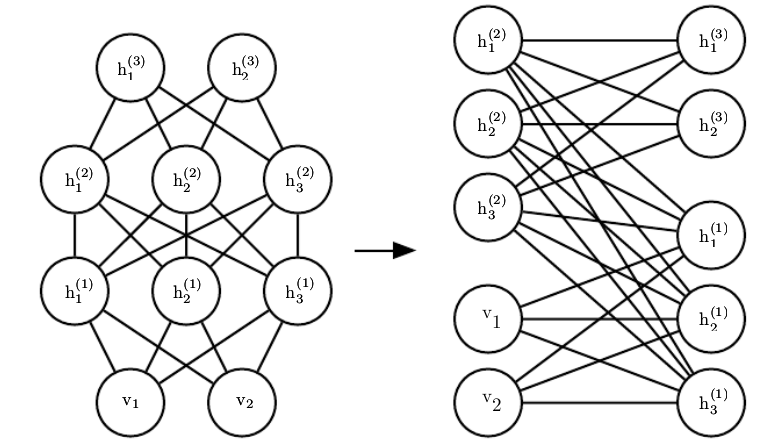
\includegraphics[scale=0.4]{img/dbm_gibbs.png}
\centering
\caption{A deep Boltzmann machine, re-arranged to reveal its bipartite graph structure.}
\label{fig:dbm_gibbs}
\end{mdframed}
\end{figure}
\textbullet{} Note that Contrastive Divergence algorithm is slow for DBMs because they do not allow efficient sampling of the hidden states given the visible units -- instead, CD would require burning in a Markov chain every time a new negative phase sample is needed.
\subsubsection{Greedy layerwise pretraining of DBMs}
DBM can be trained using the aforementioned learning algorithm from random initialization (typically the results are quite bad even on MNIST, see \cite{goodfellow2012joint, goodfellow2016deep}), but it works much better if weights are initialized sensibly. Greedy layerwise pretraining = learning procedure that consists of learning a stack of RBM's one layer at a time. After the stack is learned, the whole stack can be viewed as a single probabilistic model, called Deep Belief Net. Thus, pre-training for DBN is straightforward. In case of DBM though, a layer in the middle of the stack of RBMs is trained with only bottom-up input, but after the stack is combined to form DBM, the layer will have both bottom-up and top-down input. To account for this so-called \emph{evidence double counting problem} \cite{salakhutdinov2009deep, goodfellow2016deep}, Fig. \ref{fig:dbm_pretraining}, two modifications are required:
\begin{figure}[h]
\begin{mdframed}
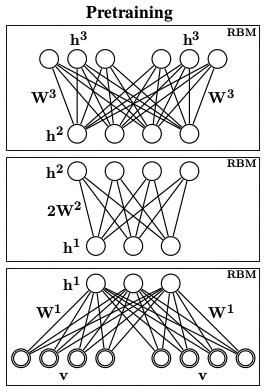
\includegraphics[width=1.5in]{img/dbm_pretraining2.png}
\quad
\quad
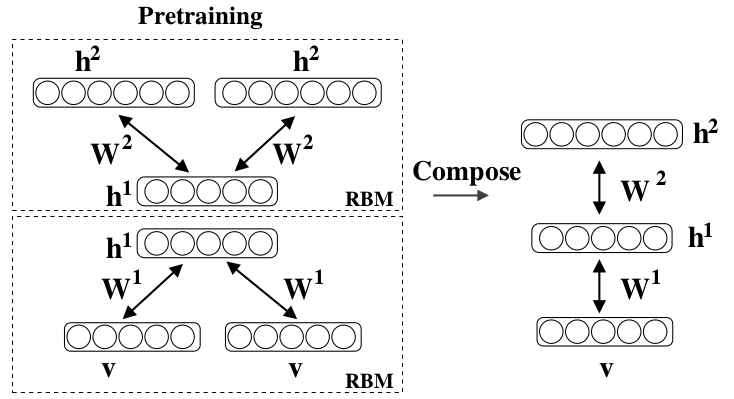
\includegraphics[width=3.5in]{img/dbm_pretraining.png}
\centering
\caption{Pre-training consists of learning a stack of modified RBMs, that are then composed to create a DBM.}
\label{fig:dbm_pretraining}
\end{mdframed}
\end{figure}
\begin{itemize}
	\item bottom RBM should be trained using two "copies" of each visible unit and the weights tied to be equal between these two copies ($\cong$ simply double the total input to hidden layer during upward pass); similarly, top RBM should be trained with two copies of topmost layer. Training of all intermediate RBMs if there are any, should not be modified.
	\item the weights of all intermediate RBMs though, should be divided by 2 before inserting into DBM
\end{itemize}
\begin{figure}[h]
\begin{mdframed}
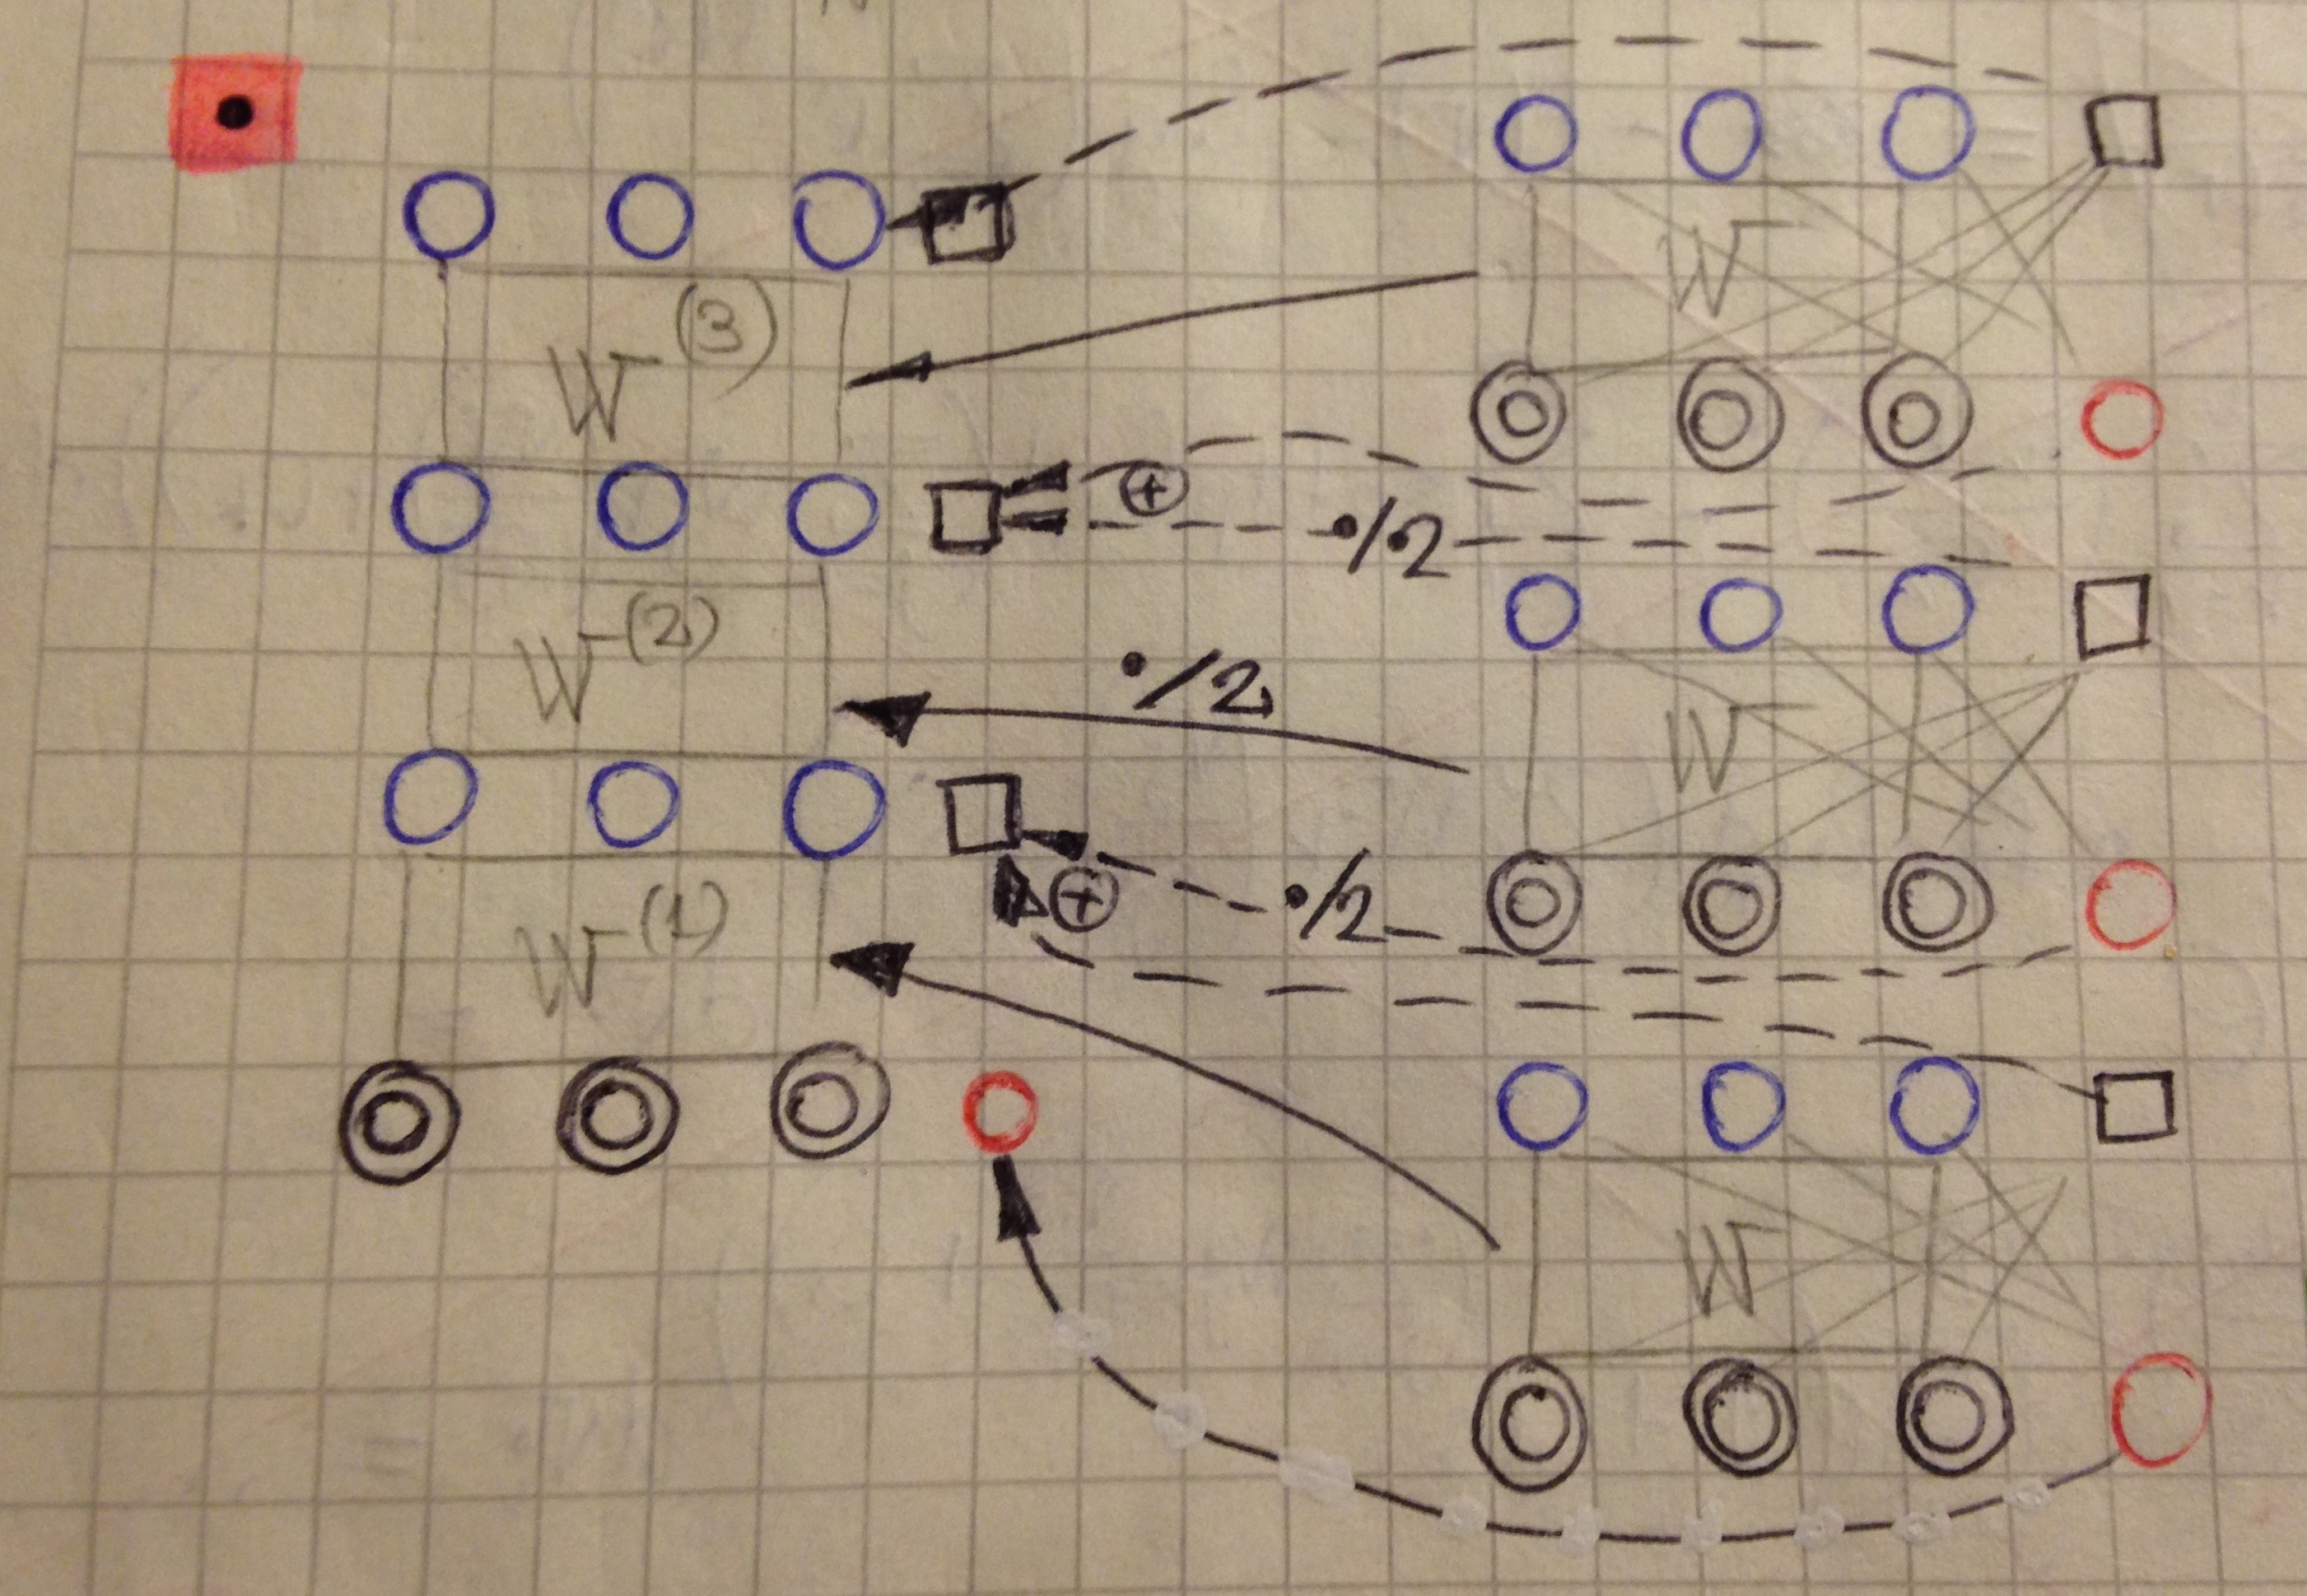
\includegraphics[scale=0.08]{dbm/dbm_init.jpg}
\centering
\caption{A more detailed scheme how to initialize 3-layer DBM from learned stack or RBMs, including biases. Black circles -- visible units, blue -- hidden units, red circel -- visible bias, black square -- hidden bias. Biases can be summed or averaged.}
\label{fig:dbm_init}
\end{mdframed}
\end{figure}

\subsubsection{Joint training of DBMs}
Classic DBMs require greedy unsupervised pretraining, and to perform classification
well, require a separate MLP-based classifier on top of the hidden features they
extract. It is hard to track performance
during training because we cannot evaluate properties of the full DBM while
training the first RBM. Software implementations
of DBMs need to have many different components for CD training of individual
RBMs, PCD training of the full DBM, and training based on back-propagation
through the MLP. Finally, the MLP on top of the Boltzmann machine loses many
of the advantages of the Boltzmann machine probabilistic model, such as being
able to perform inference when some input values are missing.
\\
There are two main ways to resolve the joint training problem of the deep
Boltzmann machine: \tb{multi-prediction DBMs}\cite{goodfellow2013multi}, which is currently beyond the scope of this project, and the \tb{centering trick} \cite{montavon2012deep}, which reparametrizes the model in order to make the Hessian of the cost function better-conditioned at the beginning of the learning process. More specifically, if we consider energy function of generalized Boltzmann Machine (BM, RBM, DBM can all be represented by appropriate choice of $\mb{x}$ -- states, $\mb{U}$ -- weights, $\mb{a}$ -- biases):
\bg
E(\mb{x};\bs{\psi})=-\mb{x}^T \mb{U}\mb{x}-\mb{a}\cdot\mb{x}
\eg
Then the idea of centering trick is simply to reparameterize this energy function as 
\bg
E(\mb{x};\bs{\psi})=-(\mb{x}-\bs{\beta})^T \mb{U}(\mb{x}-\bs{\beta})-\mb{a}\cdot(\mb{x}-\bs{\beta})
\eg
Where new hyperparameter vector $\bs{\beta}$ is chosen to be $\mb{x}-\bs{\beta}\approx \mb{0}$ at the beginning of training. This does not change the set of probability distributions that the model can represent, but it does change the learning dynamics so much, that it is actually possible to train DBM from random initialization w/o pre-training and achieve sensible results. However, in \cite{goodfellow2013multi} they say when DBM is trained using centering trick, they have never shown to have good classification performance, if this was the primary goal.

\subsubsection{Annealed importance sampling \cite{salakhutdinov2008, salakhutdinov2009deep, hinton2012better, upadhya2015empirical}}
Let $p_A(\mb{x})=\frac{p^*_A(\mb{x})}{\mc{Z}_A}$ be simple proposal distribution from which we can sample easily, and $p_{B}(\mb{x})=\frac{p^*_B(\mb{x})}{\mc{Z}_B}$ our complex target distribution. We also have to make sure $p_B \ll p_A$, which is easy in our case, since we can always choose $p_A$ to be uniform pmf, which dominates every other probability mass function on discrete units (of finite cardinality).
\\[0.5em]
\u{(Classical) Importance Sampling}
\\
The ratio of partition functions can be estimated as follows
\bg
\frac{\mc{Z}_B}{\mc{Z}_A}=\frac{p^*_B(\mb{x})}{p^*_A(\mb{x})}=\sum_{\mb{x}}\frac{p^*_B(\mb{x})}{p^*_A(\mb{x})} p_A(\mb{x})=\E_{\mb{x}\sim p_A}\l[\frac{p^*_B(\mb{x})}{p^*_A(\mb{x})} \r] \approx \frac{1}{N}\sum_{i=1}^N \frac{p^*_B(\mb{x}_i)}{p^*_A(\mb{x}_i)}
\eg
The problem is when $p_A$ and $p_B$ are very different, as in our case, this estimator is very poor: its variance is very large, possibly infinite.
\\[0.5em]
\u{Annealed Importance Sampling}
\\
To handle this issue, we define sequence of probability mass functions $\l(p_m\r)_{m=0:M}$ such that $p_0 = p_A$ and $p_M = p_B$, and for which we know unnormalized probabilities $p_m^*$, which typically are mixtures of target and proposal:
\bg
p_m(\mb{x})=p_B(\mb{x})^{\beta_m}\cdot p_A(\mb{x})^{1-\beta_m}, \beta_m=\frac{m}{M}
\eg
Also, in order not to sample from $p_s$ we also need sequence of transition operators $\l(T_i(\mb{x}_{i + 1} \leftarrow \mb{x}_i)\r)_{i=1:M-1}$ each that leaves the corresponding $p_i$ invariant. The importance weight can then be computed as
\bg
\omega_{\text{AIS}} \leftarrow \prod_{m=1}^M \frac{p_m^*(\mb{x}_m)}{p_{m-1}^*(\mb{x}_m)}
\eg
where $\mb{x}_1 \sim p_0=p_A;\; \mb{x}_2 \sim T_1(\mb{x}_2 \leftarrow \mb{x}_1);\; \ldots \; \mb{x}_M \sim T_{M-1}(\mb{x}_M \leftarrow \mb{x}_{M-1})$.
The ratio of partition functions can then be estimated as average over many AIS runs:
\bg
\frac{\mc{Z}_B}{\mc{Z}_A}=\frac{\mc{Z}_M}{\mc{Z}_0}\approx \frac{1}{L}\sum_{l=1}^L \omega_{\text{AIS}}^{(l)}
\eg
Notice also that we don't need to compute partition functions of any of the intermediate distributions.
\\
\tb{Note}: to avoid numerical problems and overflow errors (partition functions are very large numbers even for very moderate sized BM), all computations are performed in $\log$-domain, as usual.
\\[0.5em]
\u{Annealed Importance Sampling for 2-layer Bernoulli BM}
\\
It turns out that we can reduce state space of AIS to only hidden units in first layer $\mb{x}=\{\mb{h}^{(1)}\}$ by explicitly summing out visible and top-most layer hidden units:
\begin{empheq}[box={\mybox[1em][1em]}]{align*}
\log p^*\l(\mb{h}^{(1)}\r) &= \log \sum_{\mb{v},\mb{\mb{h}^{(2)}}} p^*\l(\mb{v}, \mb{h}^{(1)}, \mb{h}^{(2)}\r)=
\\
&= \log \sum_{\mb{v},\mb{\mb{h}^{(2)}}} \exp \l( \mb{v}^T\mb{W}^{(1)}\mb{h}^{(1)} +
\mb{h}^{(1)^T}\mb{W}^{(2)}\mb{h}^{(2)} + \mb{b}\cdot\mb{v} + \mb{c}^{(1)}\cdot\mb{h}^{(1)} + \mb{c}^{(2)}\cdot\mb{h}^{(2)} \r)
\\
&= \mb{c}^{(1)}\cdot\mb{h}^{(1)} + \log\l[ \sum_{\mb{v}}\exp\l( \mb{v}^T\mb{W}^{(1)}\mb{h}^{(1)} + \mb{b}\cdot\mb{v} \r)\sum_{\mb{h}^{(2)}} \exp\l( \mb{h}^{(1)^T}\mb{W}^{(2)}\mb{h}^{(2)} + \mb{c}^{(2)}\cdot\mb{h}^{(2)} \r) \r]
\\
&= \mb{c}^{(1)}\cdot\mb{h}^{(1)} + \sum_i^V \text{softplus}\l(\sum_j^{H_1} W_{ij}^{(1)}h_j^{(1)}+b_i \r) + \sum_k^{H_2} \text{softplus}\l(\sum_j^{H_1} W_{jk}^{(2)}h_k^{(2)}+c_k^{(2)} \r)
\end{empheq}
\bg
\boxed{\log p^*\l(\mb{h}^{(1)}\r)=\mb{c}^{(1)}\cdot\mb{h}^{(1)} + \sum_i^V \text{softplus}\l(\sum_j^{H_1} W_{ij}^{(1)}h_j^{(1)}+b_i \r) + \sum_k^{H_2} \text{softplus}\l(\sum_j^{H_1} W_{jk}^{(2)}h_k^{(2)}+c_k^{(2)} \r)}
\eg
From this we can easily derive equation for $\log p_{\textcolor{red}{m}}^*$ by simply scaling all weights by $\beta_m$:
\begin{equation}
\begin{aligned}
\log p_{\textcolor{red}{m}}^*\l(\mb{h}^{(1)}\r) =
\textcolor{red}{\beta_m}\mb{c}^{(1)}\cdot\mb{h}^{(1)} + \sum_i^V \text{softplus}\l(\textcolor{red}{\beta_m}\cdot\l(\sum_j^{H_1} W_{ij}^{(1)}h_j^{(1)}+b_i \r)\r) +
\\
+ \sum_k^{H_2} \text{softplus}\l(\textcolor{red}{\beta_m}\cdot\l(\sum_j^{H_1} W_{jk}^{(2)}h_k^{(2)}+c_k^{(2)} \r)\r)
\end{aligned}
\end{equation}
When $\beta_m=1$ we obtain target distribution, when $\beta_m=0$ we obtain uniform distribution:
\bg
\log p_0^*\l(\mb{h}^{(1)}\r) \equiv 0+\sum_i^V \text{softplus}(0) + \sum_k^{H_2} \text{softplus}(0)=(V+H_2)\log 2
\eg
thus $ \log \mc{Z}_0=(V+H_1+H_2)\log 2$.
\\[1em]
Thus we gradually increase "inverse temperature" $\beta$ from 0 to 1 and can estimate partition function using procedure described above. Staring from randomly initialized $\mb{h}^{(1)}$, we apply sequence of transition operators $T_i$ which are simply alternating Gibbs sampler with weights scaled by $\beta_i$.
\\[1em]
We can do the same for different types of units and larger number of layers. In the latter case we can again analytically sum out visible and top-most hidden units.
\\[0.5em]
\u{Variational lower-bound}
\\
Having estimate of partition function $\t{\mc{Z}}$, we can estimate variational lower-bound on test vector $\mb{v}^*$ as follows
\begin{equation}
\begin{aligned}
\log p(\mathbf{v}^{*};\boldsymbol{\psi})\geq\;&-\sum_{\mathbf{h}} q(\mathbf{h};\boldsymbol{\mu})E(\mathbf{v}^{*}, \mathbf{h};\boldsymbol{\psi})+\mathcal{H}(\boldsymbol{\mu})-\log\mathcal{Z}(\boldsymbol{\psi})
\\
=\;& \mathbf{v}^{*^{T}}\mathbf{W}^{(1)}\boldsymbol{\mu}_{\mathbf{v}^*}^{(1)}+\boldsymbol{\mu}_{\mathbf{v}^*}^{(1)^{T}}\mathbf{W}^{(2)}\boldsymbol{\mu}_{\mathbf{v}^*}^{(2)}+\mathbf{b}\cdot\mathbf{v}^{*}+\mathbf{c}^{(1)}\cdot\boldsymbol{\mu}_{\mathbf{v}^*}^{(1)}+\mathbf{c}^{(2)}\cdot\boldsymbol{\mu}_{\mathbf{v}^*}^{(2)}+\mathcal{H}(\boldsymbol{\mu}_{\mathbf{v}^*})-\log\mathcal{Z}(\boldsymbol{\psi})
\\
\approx\;& \mathbf{v}^{*^{T}}\mathbf{W}^{(1)}\boldsymbol{\mu}_{\mathbf{v}^*}^{(1)}+\boldsymbol{\mu}_{\mathbf{v}^*}^{(1)^{T}}\mathbf{W}^{(2)}\boldsymbol{\mu}_{\mathbf{v}^*}^{(2)}+\mathbf{b}\cdot\mathbf{v}^{*}+\mathbf{c}^{(1)}\cdot\boldsymbol{\mu}_{\mathbf{v}^*}^{(1)}+\mathbf{c}^{(2)}\cdot\boldsymbol{\mu}_{\mathbf{v}^*}^{(2)}+\mathcal{H}(\boldsymbol{\mu}_{\mathbf{v}^*})-\log\widehat{\mathcal{Z}}
\end{aligned}
\end{equation}
where $\bs{\mu}_{\mathbf{v}^*}$ are variational parameters obtained by running fixed-point equations using Gibbs sampler unitl convergence with visible units clamped to $\mathbf{v}^*$.
\\[1em]
One can also estimate true log-probability using AIS by clamping visible units to test example (estimating log-probability for one test example is computationally equivalent to estimating a partition function).

\subsubsection{Additional facts}
\textbullet{} In \cite{goodfellow2016deep} they say that obtaining sota results with DBM requires an additional partial mean field in negative phase, more details in \cite{goodfellow2013multi}.
\\
\textbullet{} The inference can further be accelerated using separate \emph{recognition model}, see \cite{salakhutdinov2010efficient} for details.
\\
\textbullet{} DBMs were developed after DBNs. Compared to DBNs, the posterior distribution $p(\mb{h}|\mb{v})$ is simpler for DBMs. Somewhat counterintuitively, the simplicity of this posterior distribution allows richer approximations of the posterior \cite{goodfellow2016deep}
\\
\textbullet{} The use of proper mean field allows the approximate inference procedure for DBMs to capture the influence of top-down feedback interactions. This makes
DBMs interesting from the point of view of neuroscience, because the human brain
is known to use many top-down feedback connections\cite{goodfellow2016deep}.
\\
\textbullet{} In \cite{goodfellow2013joint} they observe that energy function $E(\mb{v},\mb{h};\bs{\psi})$ inevitably induces some prior $p(\mb{h};\bs{\psi})$ that is not motivated by the structure of any kind of data. The role of deeper layers in DBM is simply to provide a better prior on the first layer hidden units.

\clearpage
\begin{figure}[h]
\begin{mdframed}
\centering
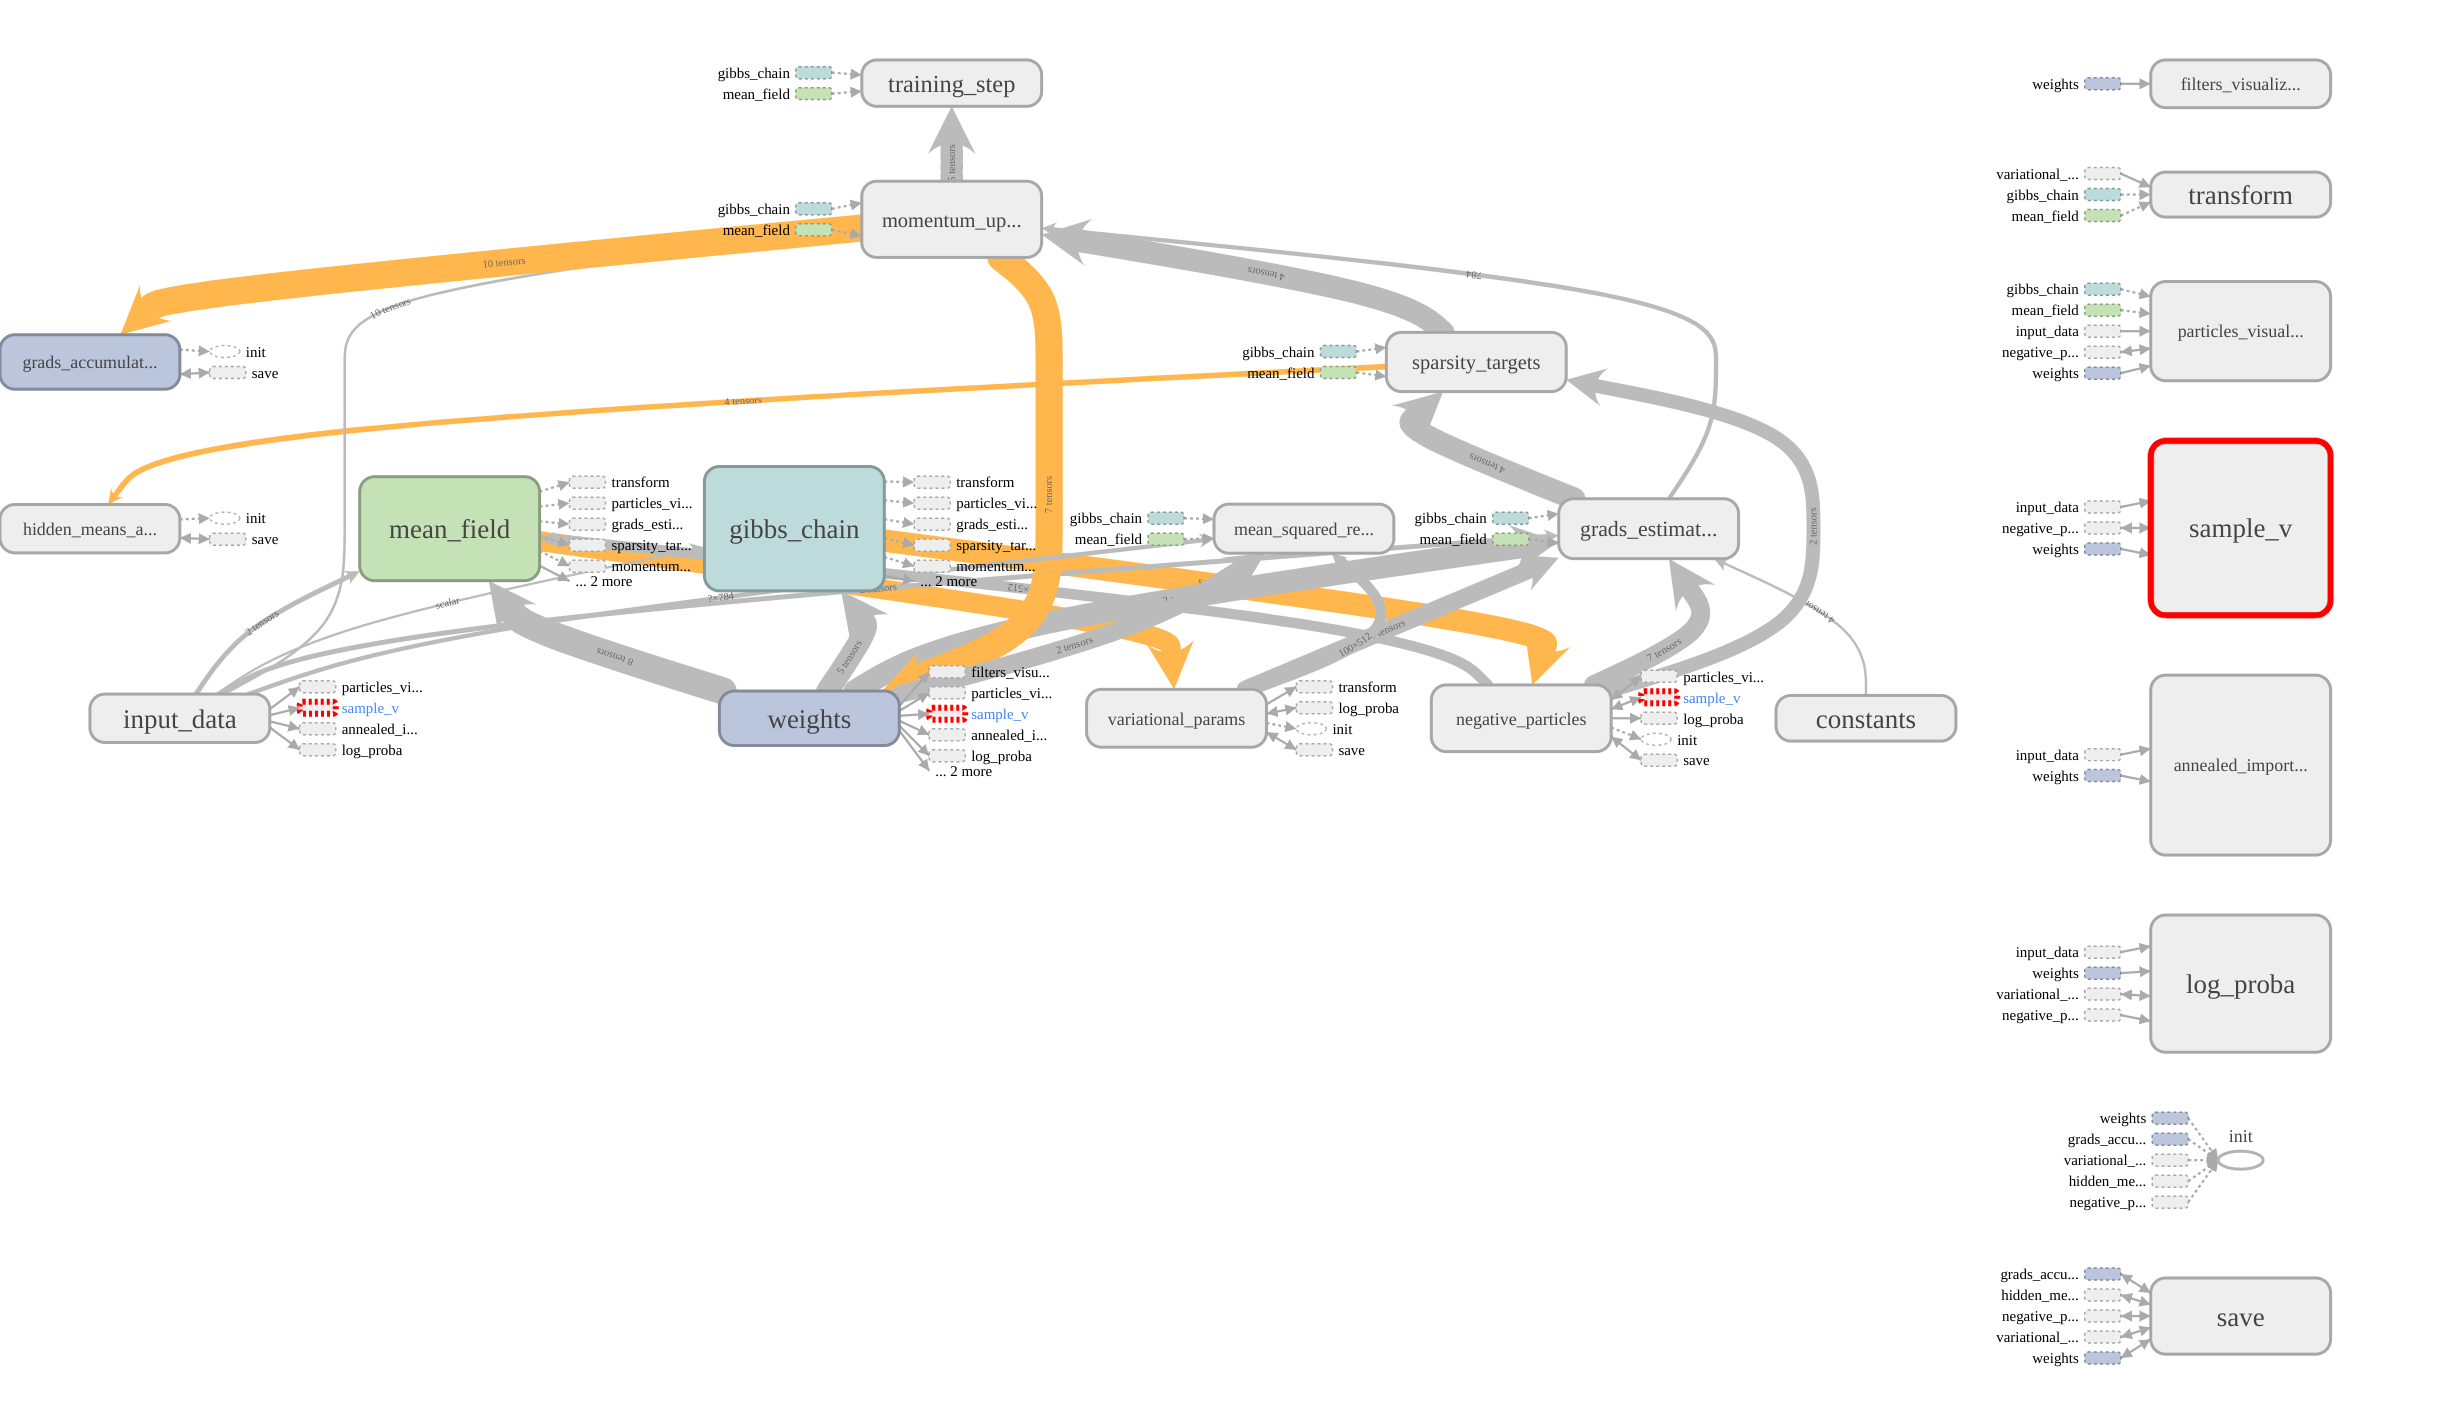
\includegraphics[width=6.4in]{dbm/tf_graph.png}
\caption{High-level computational graph for DBM model.}
\end{mdframed}
\end{figure}
